\chapter{Présentation du projet}
\section{Sujet}
Le problème a N-corps consiste à calculer le mouvement de  N particules en connaissant leur masse et leur vitesse respective.
Il s'agit donc de résoudre les équations du mouvement de Newton pour ces N particules.
Le problème à N-corps est une simulation classique et importante pour l'astronomie, étant donné qu'il permet d'étudier la mécanique de corps céleste interagissant gravitationnellement.
Le problème à deux corps et le problème à trois sont  résolubles analytiquement. Pour N>3, il n'existe pas de résolution analytique, il faut donc utiliser des solutions approchées.

%inclusion d'une mage dans le document
\begin{figure}[!h]
\begin{center}
%taille de l'image en largeur
%remplacer "width" par "height" pour régler la hauteur
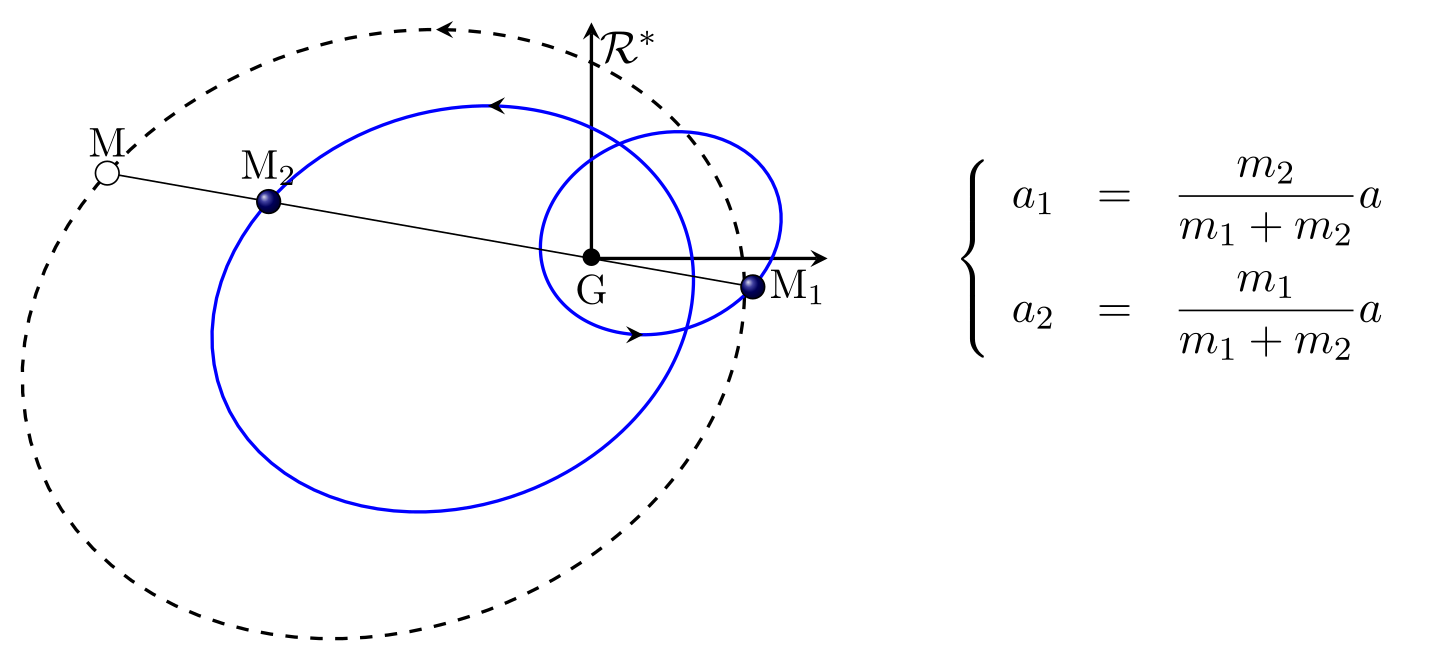
\includegraphics[width=13cm]{presentation/2_corps.png}
\end{center}
%légende de l'image
\captionsetup{hypcap=false}
\caption{Solution du problème à 2 corps}
\label{fig1}
\end{figure}

\section{Objectif : résolution la plus efficace possible du problème à N-corps}

L'objectif du projet est donc de résoudre le plus efficacement possible le problème à n-corps afin de simuler par exemple des galaxies.
Pour cela, nous utiliserons des solutions approchées calculées à partir de l'algorithme de Barnes-Hut. Nous étudierons également l'application de la parallélisation à notre programme.
En pratique, le projet consiste à continuer et améliorer un projet déjà bien entamé afin d'acquérir de nouvelles compétences en C++, sur les algorithmes hiérarchiques , en parallélisation et plus généralement en optimisation de code.

\section{Démarche}

Un code C++ implémentant une interface graphique nous a été fourni pour le projet.
Nous allons dans un premier temps calculer la force qui s'applique à chaque particules à partir de la formule de l'interaction gravitationnelle. La position se calcule alors en utilisant un intégrateur numérique (Méthode d'Euler, saute mouton...).
Dans un deuxième temps, nous utiliserons l'algorithme de Barnes-Hut pour le calcul des forces.
Enfin, nous utiliserons la parallélisation multi-thread pour accélérer nos calculs.
